\chapter{Poisson-Klammern, Erzeuger und Drehimpuls}

\lectureoverview{Die Poisson-Klammer ist mehr als eine kompakte Schreibweise für die Hamilton-Gleichungen. Sie ist eine algebraische Operation, die Transformationen erzeugt. Die Klammerung mit dem Hamiltonian erzeugt die Zeitentwicklung, die mit dem Impuls Translationen und die mit dem Drehimpuls Drehungen. In dieser Sprache werden Symmetrie und Erhaltung zu zwei Lesarten derselben verschwindenden Klammer. Wir entwickeln diesen Gedanken am harmonischen Oszillator und nutzen anschließend die Drehimpulsalgebra, um die gyroskopische Präzession herzuleiten, ohne Euler-Winkel einzuführen.}

\section{Eine Funktion entlang einer Hamiltonschen Trajektorie}

Sei \[
  F=F(q_1,\ldots,q_n,p_1,\ldots,p_n)
\] eine hinreichend differenzierbare Funktion auf dem Phasenraum. Man kann sie auf zwei Arten betrachten. Erstens ordnet sie jedem Punkt des Phasenraums eine Zahl zu. Zweitens wird sie, sobald eine Hamiltonsche Trajektorie gewählt ist, zu einer Funktion der Zeit, weil sich der Punkt \((q(t),p(t))\) bewegt. Entlang dieser Trajektorie gilt \begin{equation}
  \frac{dF}{dt}
  =
  \sum_i\left(
    \frac{\partial F}{\partial q_i}\dot q_i
    +\frac{\partial F}{\partial p_i}\dot p_i
  \right).
  \label{eq:l8-chain-rule}
\end{equation} Die Hamilton-Gleichungen \begin{equation}
  \dot q_i=\frac{\partial H}{\partial p_i},
  \qquad
  \dot p_i=-\frac{\partial H}{\partial q_i},
  \label{eq:l8-hamilton-equations}
\end{equation} führen zu \begin{equation}
  \frac{dF}{dt}
  =
  \sum_i\left(
    \frac{\partial F}{\partial q_i}
    \frac{\partial H}{\partial p_i}
    -
    \frac{\partial F}{\partial p_i}
    \frac{\partial H}{\partial q_i}
  \right).
  \label{eq:l8-fdot-expanded}
\end{equation} Die rechte Seite tritt in der klassischen Mechanik häufig auf, auch wenn keiner ihrer beiden Einträge der Hamiltonian ist. Das legt folgende Definition nahe: \begin{equation}
  \boxed{
  \{F,G\}
  =
  \sum_i\left(
    \frac{\partial F}{\partial q_i}
    \frac{\partial G}{\partial p_i}
    -
    \frac{\partial F}{\partial p_i}
    \frac{\partial G}{\partial q_i}
  \right).}
  \label{eq:l8-poisson-definition}
\end{equation} Gleichung~\eqref{eq:l8-fdot-expanded} lautet damit \begin{equation}
  \boxed{\dot F=\{F,H\}.}
  \label{eq:l8-time-generator}
\end{equation}

\begin{classroomqa}
  \audiencequestion{Wenn der zweite Eintrag von \(H\) auf eine beliebige Funktion \(G\) geändert wird, ist die Klammer dann weiterhin die Zeitableitung von \(F\)?\lecturetimestamp{00:05:45--00:06:15}}
  \lecturerresponse{Nein. Während die Notation verallgemeinert wird, erkennt das Publikum einen wichtigen Punkt. Gleichung~\eqref{eq:l8-poisson-definition} definiert \(\{F,G\}\) für zwei beliebige Phasenraumfunktionen, aber \(\dot F=\{F,G\}\) gilt nur, wenn \(G\) der Hamiltonian ist. Ein allgemeines \(G\) erzeugt eine andere infinitesimale Transformation.}
\end{classroomqa}

Eine kleine Zeitänderung lässt sich zweckmäßig schreiben als
\begin{equation}
  \delta_t F=\epsilon\,\{F,H\}.
  \label{eq:l8-small-time-step}
\end{equation}
Diese Form nimmt das Folgende vorweg. Die Zeitentwicklung ist ein Mitglied einer größeren Familie von Transformationen, die durch Poisson-Klammern erzeugt werden.

\section{Die Algebra der Klammern}

Die Klammer lässt sich nun als eigene Art der Differenzialrechnung verwenden. Ihre Regeln folgen aus der gewöhnlichen Differentiation:
\begin{align}
  \{A,B\}&=-\{B,A\}, \label{eq:l8-antisymmetry}\\
  \{A+B,C\}&=\{A,C\}+\{B,C\}, \label{eq:l8-additivity}\\
  \{\lambda A,B\}&=\lambda\{A,B\},
    \quad \lambda\ \text{constant}, \label{eq:l8-scalar-rule}\\
  \{AB,C\}&=A\{B,C\}+\{A,C\}B. \label{eq:l8-leibniz}
\end{align}
Diese vier Zeilen drücken der Reihe nach Antisymmetrie, Additivität, Linearität bei Multiplikation mit einer Konstanten und die Leibniz-Regel aus. Phasenraumfunktionen der klassischen Mechanik sind unter der gewöhnlichen Multiplikation kommutativ; daher ist die Anordnung der gewöhnlichen Faktoren \(A\) und \(B\) in der letzten Zeile unerheblich. Für Operatoren in der Quantenmechanik gilt das nicht mehr. Aus der Antisymmetrie folgt außerdem
\begin{equation}
  \{A,A\}=0.
  \label{eq:l8-self-bracket}
\end{equation}

Für kanonische Koordinaten lauten die elementaren Klammern
\begin{equation}
  \boxed{
  \{q_i,q_j\}=0,\qquad
  \{p_i,p_j\}=0,\qquad
  \{q_i,p_j\}=\delta_{ij}.}
  \label{eq:l8-canonical-brackets}
\end{equation}
Jede Funktion, die nur von den \(q_i\) abhängt, hat mit jeder anderen Funktion, die nur von den \(q_i\) abhängt, eine verschwindende Klammer. Entsprechendes gilt für Funktionen, die nur von den \(p_i\) abhängen. Eine Klammer ist nur dann von null verschieden, wenn eine kanonische Koordinate auf ihren konjugierten Impuls trifft. Das Kronecker-Delta in Gl.~\eqref{eq:l8-canonical-brackets} hält fest, dass nur übereinstimmende Indizes zusammentreffen.

\subsection{Der harmonische Oszillator als Prüfstein}

Betrachten wir
\begin{equation}
  H=\frac{p^2}{2m}+\frac{kq^2}{2}.
  \label{eq:l8-oscillator-hamiltonian}
\end{equation}
Nun verwenden wir bewusst nur die Klammerregeln und Gl.~\eqref{eq:l8-time-generator}. Zunächst gilt
\begin{align}
  \dot q
  &=\{q,H\}\\
  &=\frac{1}{2m}\{q,p^2\}\\
  &=\frac{1}{2m}\left(p\{q,p\}+\{q,p\}p\right)\\
  &=\frac{p}{m}.
  \label{eq:l8-qdot-oscillator}
\end{align}
Der Potentialterm fällt weg, weil \(\{q,q^2\}=0\). Entsprechend gilt
\begin{align}
  \dot p
  &=\{p,H\}\\
  &=\frac{k}{2}\{p,q^2\}\\
  &=\frac{k}{2}\left(q\{p,q\}+\{p,q\}q\right)\\
  &=-kq.
  \label{eq:l8-pdot-oscillator}
\end{align}
Das Minuszeichen ergibt sich genau aus der Antisymmetrie \(\{p,q\}=-\{q,p\}=-1\). Durch Kombination der beiden Gleichungen erster Ordnung erhalten wir
\begin{equation}
  m\ddot q=-kq.
  \label{eq:l8-hooke-equation}
\end{equation}

\begin{figure}[htbp]
  \centering
  
\includegraphics[width=0.82\textwidth]{lecture_08_figure_01.png}
  \caption{Der Oszillator-Hamiltonian und die beiden Klammerberechnungen, aus denen \(\dot q=p/m\) und \(\dot p=-kq\) hervorgehen.}
  \lectureframe{00:23:20}
\end{figure}

Während der Rechnung sucht die Klasse nach einem Verb für \emph{eine Poisson-Klammer bilden} und einigt sich vorläufig auf \emph{poissonieren}. Der Scherz markiert einen echten Perspektivwechsel: Ist die Algebra erst einmal bekannt, kann man direkt mit ihr rechnen, statt jedes Ergebnis aus der Definition neu herzuleiten.

\begin{classroomqa}
  \audiencequestion{Ist diese mathematische Struktur eine Gruppe oder eine Algebra? Gibt es Inverse? \lecturetimestamp{00:23:48--00:24:16}}
  \lecturerresponse{Sie ist keine Gruppe: Die Klammeroperation liefert weder das erforderliche neutrale Element noch Inverse. Die Phasenraumfunktionen bilden eine Poisson-Algebra: Sie verfügen über gewöhnliche kommutative Multiplikation und Addition sowie über eine antisymmetrische Klammer, die der Leibniz-Regel genügt. Eine weitere Identität, die Jacobi-Identität, vervollständigt die übliche abstrakte Definition, wird in dieser Vorlesung jedoch nicht entwickelt.}
\end{classroomqa}

\begin{classroomqa}
  \audiencequestion{Wie hängen Poisson-Klammern und Quantenkommutatoren zusammen? \lecturetimestamp{00:24:18--00:25:00}}
  \lecturerresponse{Die Vorlesung gibt dazu nur einen Ausblick. Beim Übergang zur Quantenmechanik wird die klassische Klammer schematisch ersetzt durch
  \[
    \{A,B\}_{\mathrm{PB}}
    \longleftrightarrow
    \frac{1}{i\hbar}[\widehat A,\widehat B].
  \]
  Diese Zuordnung erfordert Einschränkungen hinsichtlich der Operatorordnung und Quantisierung; hier wird sie nicht als Satz verwendet.}
\end{classroomqa}

Beim Oszillator hat die Klammer lediglich die Hamilton-Gleichungen wiederhergestellt. Ihre eigentliche Stärke zeigt sich, wenn der Erzeuger eine andere Erhaltungsgröße als \(H\) ist.

\section{Der Drehimpuls aus der Rotationssymmetrie}

Zur Erinnerung: Früher im Kurs haben wir die infinitesimale Form der Noether-Konstruktion verwendet. Ändert eine kontinuierliche Symmetrie die Koordinaten gemäß
\begin{equation}
  \delta q_i=\epsilon F_i(q),
  \label{eq:l8-noether-variation}
\end{equation}
so lautet die zugehörige Erhaltungsgröße in der hier betrachteten Situation
\begin{equation}
  G=\sum_i p_iF_i(q).
  \label{eq:l8-noether-charge}
\end{equation}
Der Gesamtfaktor \(\epsilon\) kann weggelassen werden: Multipliziert man eine Erhaltungsgröße mit einer festen Zahl, ändert sich das Erhaltungsgesetz nicht.

Drehen wir ein Teilchen infinitesimal um die \(z\)-Achse. Bei der in der Vorlesung verwendeten Orientierung gilt
\begin{equation}
  \delta x=-\epsilon y,\qquad
  \delta y=\epsilon x,\qquad
  \delta z=0.
  \label{eq:l8-z-rotation}
\end{equation}
Gl.~\eqref{eq:l8-noether-charge} ergibt
\begin{equation}
  L_z=-p_xy+p_yx=xp_y-yp_x.
  \label{eq:l8-lz}
\end{equation}
Durch zyklisches Vertauschen von \(x\), \(y\) und \(z\) erhalten wir
\begin{equation}
  \boxed{\begin{aligned}
    L_x&=yp_z-zp_y,\\
    L_y&=zp_x-xp_z,\\
    L_z&=xp_y-yp_x.
  \end{aligned}}
  \label{eq:l8-angular-components}
\end{equation}
Dies sind die Komponenten von
\begin{equation}
  \boldsymbol L=\boldsymbol r\times\boldsymbol p.
  \label{eq:l8-cross-product}
\end{equation}

\begin{figure}[htbp]
  \centering
  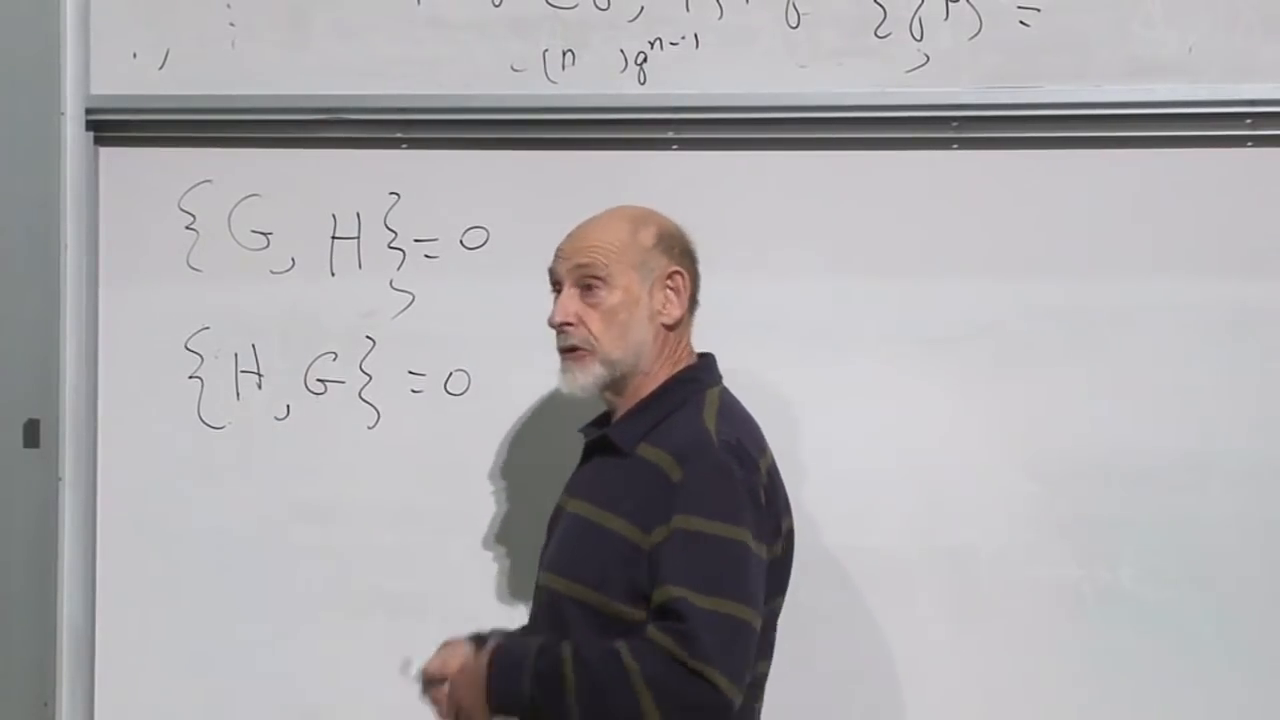
\includegraphics[width=0.82\textwidth]{lecture_08_figure_02.png}
  \caption{Die drei kartesischen Komponenten des Drehimpulses und ihre kompakte Darstellung als Kreuzprodukt.}
  \lectureframe{00:34:00}
\end{figure}

Eine Drehung um einen beliebigen Einheitsvektor \(\boldsymbol n\) wird erzeugt durch
\begin{equation}
  L_{\boldsymbol n}=\boldsymbol n\cdot\boldsymbol L.
  \label{eq:l8-arbitrary-axis}
\end{equation}
Für ein isoliertes rotationsinvariantes System sind alle drei Komponenten erhalten. Bleiben nur Drehungen um eine Achse symmetrisch, so ist nur die Komponente entlang dieser Achse sicher erhalten.

\section{Der Drehimpuls erzeugt Drehungen}

Anstatt sofort ein Problem der Rotationsdynamik zu lösen, untersuchen wir zunächst, was \(L_z\) unter der Klammer bewirkt. Mit Gl.~\eqref{eq:l8-lz} gilt
\begin{align}
  \{x,L_z\}
  &=\{x,xp_y-yp_x\}
   =-y\{x,p_x\}
   =-y,\\
  \{y,L_z\}
  &=\{y,xp_y-yp_x\}
   =x\{y,p_y\}
   =x,\\
  \{z,L_z\}&=0.
  \label{eq:l8-position-rotation-brackets}
\end{align}
Dies sind genau die Koeffizienten aus Gl.~\eqref{eq:l8-z-rotation}.

\begin{figure}[htbp]
  \centering
  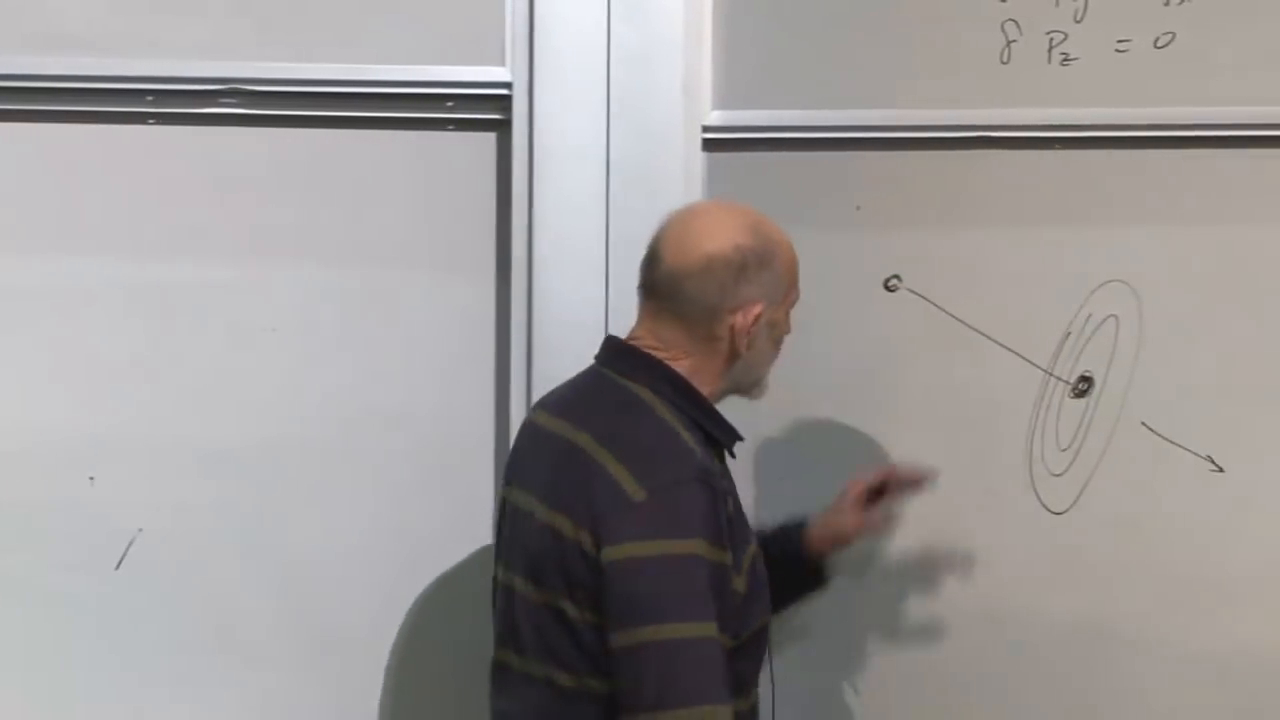
\includegraphics[width=0.82\textwidth]{lecture_08_figure_03.png}
  \caption{Die Koordinatenklammern mit \(L_z\): Die Klammer reproduziert die infinitesimale Drehung von \((x,y,z)\).}
  \lectureframe{00:38:41}
\end{figure}

Auch der Impuls ist ein Vektor, und dieselbe Rechnung ergibt
\begin{equation}
  \begin{aligned}
    \{p_x,L_z\}&=-p_y,\\
    \{p_y,L_z\}&=p_x,\\
    \{p_z,L_z\}&=0.
  \end{aligned}
  \label{eq:l8-momentum-rotation-brackets}
\end{equation}

\begin{figure}[htbp]
  \centering
  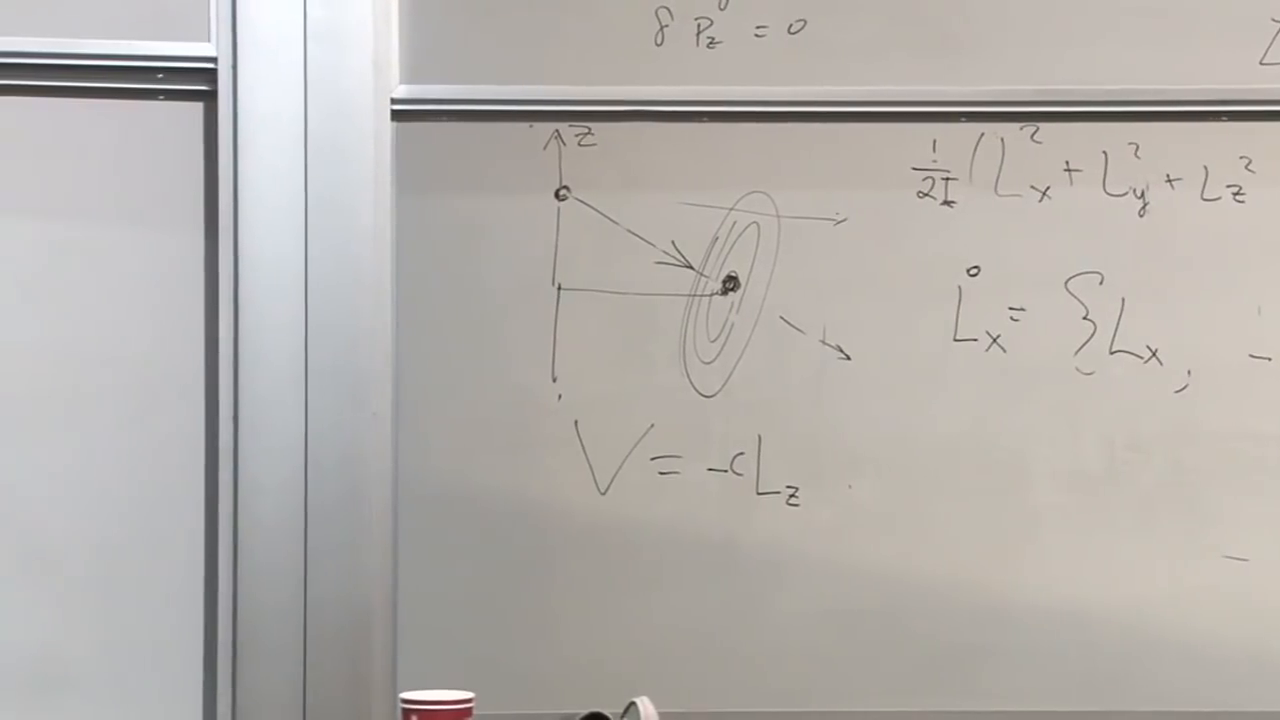
\includegraphics[width=0.82\textwidth]{lecture_08_figure_04.png}
  \caption{Ort und Impuls transformieren sich unter der von \(L_z\) erzeugten Drehung nach demselben Vektormuster.}
  \lectureframe{00:42:08}
\end{figure}

Die allgemeine Hamiltonsche Aussage lautet somit
\begin{equation}
  \boxed{\delta_G A=\epsilon\{A,G\}.}
  \label{eq:l8-generator-rule}
\end{equation}
Jede Phasenraumfunktion \(G\) definiert eine solche infinitesimale kanonische Transformation. Für \(G=L_z\) handelt es sich um eine Drehung. Für \(G=H\) ist sie ein kleiner Zeitschritt.

\begin{classroomqa}
  \audiencequestion{In der Vorlesung ist manchmal davon die Rede, das System zu drehen, und manchmal davon, die Koordinaten zu drehen. Welche Konvention gilt in den Klammergleichungen? \lecturetimestamp{00:28:22--00:29:35}}
  \lecturerresponse{Gl.~\eqref{eq:l8-z-rotation} legt die Konvention fest: Sie beschreibt die infinitesimale aktive Drehung \((x,y)\mapsto(x-\epsilon y,y+\epsilon x)\). Bei einer passiven Drehung der Achsen kehrt sich das Vorzeichen um. Ist die Konvention einmal festgelegt, sind die Klammerformeln eindeutig.}
\end{classroomqa}

\section{Der Impuls erzeugt Translationen}

Eine Translation in einer Koordinate hat die Form
\begin{equation}
  \delta q=\epsilon.
  \label{eq:l8-q-translation}
\end{equation}
Hier gilt \(F(q)=1\) in Gl.~\eqref{eq:l8-noether-variation}, daher ist die zugehörige Erhaltungsgröße \(p\). Die Behauptung, dass diese Größe die Transformation erzeugt, sagt voraus:
\begin{equation}
  \{f(q),p\}=\frac{df}{dq}.
  \label{eq:l8-translation-derivative}
\end{equation}
In der Vorlesung wird dies zunächst für Potenzen durch vollständige Induktion bewiesen. Der Induktionsanfang lautet \(\{q,p\}=1\). Es sei
\begin{equation}
  \{q^{n-1},p\}=(n-1)q^{n-2}.
  \label{eq:l8-induction-hypothesis}
\end{equation}
Dann liefert die Produktregel
\begin{align}
  \{q^n,p\}
  &=\{q\,q^{n-1},p\}\\
  &=q\{q^{n-1},p\}+\{q,p\}q^{n-1}\\
  &=(n-1)q^{n-1}+q^{n-1}\\
  &=nq^{n-1}.
  \label{eq:l8-power-translation}
\end{align}
Durch Linearität lässt sich das Ergebnis auf Polynome und konvergente Potenzreihendarstellungen erweitern. Unmittelbarer ergibt sich aus der Definition der Klammer Gl.~\eqref{eq:l8-translation-derivative} für jede differenzierbare Funktion \(f(q)\):
\begin{equation}
  \{f(q),p\}
  =
  \frac{\partial f}{\partial q}
  \frac{\partial p}{\partial p}
  =f'(q).
\end{equation}

\begin{figure}[htbp]
  \centering
  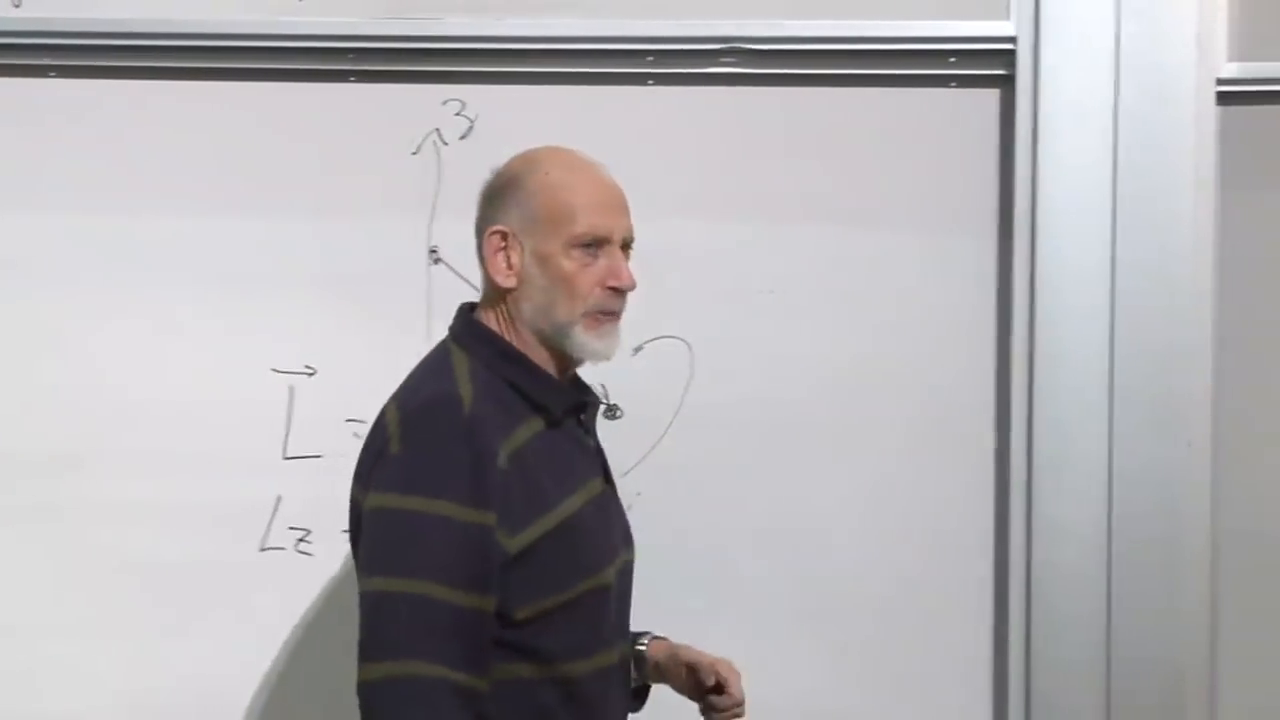
\includegraphics[width=0.82\textwidth]{lecture_08_figure_05.png}
  \caption{Das Translationsresultat nach dem Induktionsbeweis:
  \(\{F(q),p\}=dF/dq\).}
  \lectureframe{00:53:18}
\end{figure}

Wir haben nun drei Ausprägungen desselben Gedankens gesehen:
\begin{center}
  \begin{tabular}{@{}>{\raggedright\arraybackslash}p{0.37\textwidth}
                      >{\raggedright\arraybackslash}p{0.55\textwidth}@{}}
    \toprule
    Erzeuger und Transformation & Infinitesimale Wirkung\\
    \midrule
    \(H\), Zeittranslation & \(\delta_tA=\epsilon\{A,H\}\)\\
    \(p_i\), räumliche Translation & \(\delta A=\epsilon\{A,p_i\}\)\\
    \(L_i\), Drehung & \(\delta A=\epsilon\{A,L_i\}\)\\
    \bottomrule
  \end{tabular}
\end{center}
Die einer kontinuierlichen Symmetrie zugeordnete Erhaltungsgröße ist zugleich der Erzeuger dieser Symmetrie.

\section{Eine Klammer, zwei Lesarten}

Sei \(G(q,p)\) ein vorgeschlagener Erzeuger. Ist er erhalten und hängt nicht explizit von der Zeit ab, dann gilt
\begin{equation}
  \dot G=\{G,H\}=0.
  \label{eq:l8-g-conserved}
\end{equation}
Aufgrund der Antisymmetrie gilt
\begin{equation}
  \{H,G\}=0.
  \label{eq:l8-h-invariant}
\end{equation}
Die Gleichungen sind mathematisch gleichwertig, haben aber unterschiedliche physikalische Bedeutungen:
\begin{itemize}
  \item \(\{G,H\}=0\)besagt, dass \(G\) sich unter der von \(H\) erzeugten Zeitentwicklung nicht ändert.
  \item \(\{H,G\}=0\)besagt, dass \(H\) sich unter der von \(G\) erzeugten Transformation nicht ändert.
\end{itemize}
Die erste Gleichung ist ein Erhaltungsgesetz, die zweite eine Symmetrie des Hamiltonians. Noethers Zusammenhang ist in einer einzigen Null zusammengefasst.

\begin{figure}[htbp]
  \centering
  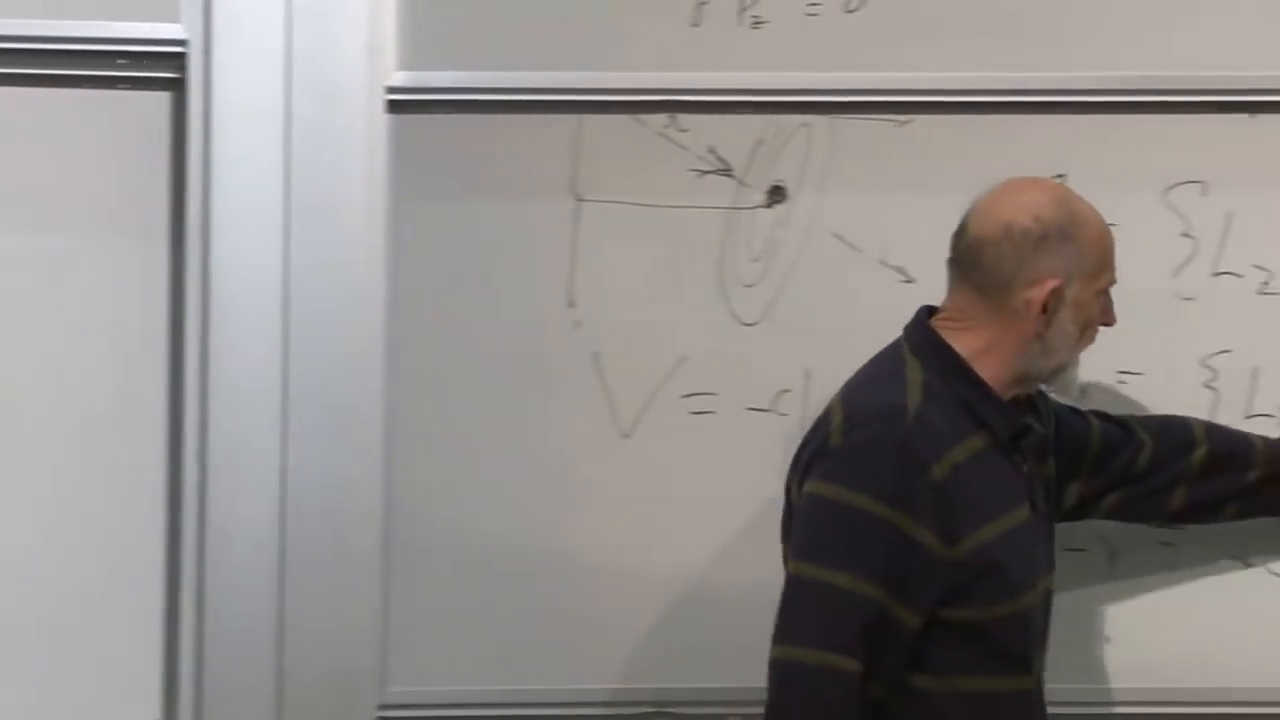
\includegraphics[width=0.82\textwidth]{lecture_08_figure_06.png}
  \caption{Die beiden Anordnungen derselben verschwindenden Klammer: Erhaltung von \(G\) und Invarianz von \(H\) unter der von \(G\) erzeugten Transformation.}
  \lectureframe{01:03:05}
\end{figure}

\begin{classroomqa}
  \audiencequestion{Lässt sich die zugehörige Symmetrie immer rekonstruieren, wenn eine Erhaltungsgröße bekannt ist? \lecturetimestamp{01:01:42--01:02:15}}
  \lecturerresponse{Im Rahmen dieser Hamiltonschen Beschreibung: ja. Man bildet die Klammer jeder Phasenraumvariablen mit \(G\). Die Gesamtheit \(\delta_GA=\epsilon\{A,G\}\) gibt an, wie sich die Variablen transformieren. Die Klammern mit \(L_z\) zeigen beispielsweise eine Drehung, selbst wenn diese Deutung zuvor nicht bekannt war. In weiterführenden Zusammenhängen können globale und Randprobleme auftreten; hier wird jedoch die lokale infinitesimale Aussage verwendet.}
\end{classroomqa}

\begin{classroomqa}
  \audiencequestion{Beschreiben diese Klammergleichungen die physikalische Bewegung, die für die Erhaltung verantwortlich ist?\lecturetimestamp{00:56:01--00:58:13}}
  \lecturerresponse{Nein. Sie identifizieren die Symmetrietransformation, nicht die tatsächliche Trajektorie. Die Erhaltung von \(L_z\) weist auf Rotationssymmetrie hin; sie besagt nicht, dass sich das Teilchen auf einer Kreisbahn bewegt. Die tatsächliche Zeitentwicklung wird von \(H\) erzeugt. Eine Klammer mit einem anderen Erzeuger beschreibt eine andere Transformationsrichtung im Phasenraum.}
\end{classroomqa}

\begin{classroomqa}
  \audiencequestion{Gibt es eine allgemeine Aussage über Transformationen, die Erhaltung nicht bereits voraussetzt? \lecturetimestamp{01:02:40--01:04:45}}
  \lecturerresponse{Ja. Gleichung~\eqref{eq:l8-generator-rule} definiert für jede Funktion \(G\) eine infinitesimale Transformation, unabhängig davon, ob sie erhalten ist. Zur Symmetrie wird sie erst, wenn der Hamiltonian invariant ist:
  \(\{H,G\}=0\). Liest man dieselbe Bedingung in umgekehrter Reihenfolge, besagt sie dann, dass \(G\) erhalten ist.}
\end{classroomqa}

\section{Die Drehimpulsalgebra}

Mit der nächsten Rechnung müssen wir die Teilchenkoordinaten nicht mehr bei jedem Rotationsproblem mitführen. Wir beginnen mit
\[
  L_x=yp_z-zp_y,\qquad
  L_z=xp_y-yp_x.
\]
In \(\{L_x,L_z\}\) verschwinden die meisten Kreuzterme, weil ihre Indizes keine kanonischen Paare bilden. Die verbleibenden Kontraktionen ergeben
\begin{align}
  \{L_x,L_z\}
  &=\{yp_z-zp_y,xp_y-yp_x\}\\
  &=xp_z-zp_x\\
  &=-L_y.
  \label{eq:l8-lx-lz}
\end{align}
Bei umgekehrter Reihenfolge entfällt das Minuszeichen. Durch zyklisches Vertauschen der Koordinaten erhalten wir
\begin{equation}
  \boxed{\begin{aligned}
    \{L_x,L_y\}&=L_z,\\
    \{L_y,L_z\}&=L_x,\\
    \{L_z,L_x\}&=L_y.
  \end{aligned}}
  \label{eq:l8-angular-algebra}
\end{equation}
In Indexschreibweise:
\begin{equation}
  \{L_i,L_j\}=\varepsilon_{ijk}L_k.
  \label{eq:l8-angular-algebra-index}
\end{equation}

\begin{figure}[htbp]
  \centering
  \includegraphics[width=0.82\textwidth]{lecture_08_figure_07.png}
  \caption{Die zyklische Poisson-Klammer-Algebra der drei Drehimpulskomponenten.}
  \lectureframe{01:10:52}
\end{figure}

Das Ergebnis hätte sich auch vorhersagen lassen. Da \(\boldsymbol L\) ein Vektor ist, muss die Klammer seiner \(x\)-Komponente mit \(L_z\) die infinitesimale Änderung dieser Komponente unter einer Drehung um die \(z\)-Achse ergeben, also \(-L_y\). Die explizite Rechnung bestätigt dieses geometrische Argument. Diese Gleichungen sind außerdem die klassischen Vorläufer der quantenmechanischen Drehimpuls-Kommutationsrelationen.

\section{Ein schnell rotierendes Gyroskop}

Betrachten wir als Anwendung ein Gyroskop: ein schnell rotierendes Schwungrad, dessen Mittelpunkt einen festen Abstand \(R\) von einem Drehpunkt hat. Der Vektor \(\boldsymbol r\) zeigt vom Drehpunkt zum Mittelpunkt des Schwungrads. Das Schwungrad dreht sich so schnell um seine Achse, dass der dominante Drehimpuls entlang dieser Richtung ausgerichtet bleibt. In der Näherung der Vorlesung gilt
\begin{equation}
  \boldsymbol L=\ell\,\boldsymbol r,
  \qquad
  L_z=\ell z,
  \label{eq:l8-L-parallel-r}
\end{equation}
Dabei wird \(\ell=L/R\) als konstant behandelt. Kleinere Drehimpulse, die mit Nutation oder einer Bewegung der Achse verbunden sind, werden zunächst vernachlässigt.

\begin{figure}[htbp]
  \centering
  \begin{tikzpicture}[scale=0.95,>=Latex]
    \coordinate (P) at (0,3.2);
    \coordinate (C) at (3.7,1.55);
    \draw[->] (0,-0.2) -- (0,4.35) node[above] {\(z\)};
    \fill (P) circle (1.7pt) node[left] {pivot};
    \draw[very thick,->] (P) -- (C)
      node[midway,above right] {\(\boldsymbol r\parallel\boldsymbol L\)};
    \fill (C) circle (1.7pt);
    \draw[dashed] (P) -- (0,1.55);
    \draw[dashed] (0,1.55) -- (C);
    \node[left] at (0,1.55) {\(z\)};
    \begin{scope}[shift={(C)},rotate=-24]
      \draw[very thick] (0,0) ellipse (0.65 and 1.35);
      \draw[thick] (0,0) ellipse (0.42 and 0.9);
    \end{scope}
    \draw[->,thick] (2.15,2.85)
      arc[start angle=140,end angle=35,radius=1.65];
  \end{tikzpicture}
  \caption{Näherung für ein schnell rotierendes Gyroskop. Der Abstand zwischen Drehpunkt und Mittelpunkt ist fest, und der dominante Drehimpuls der Rotation bleibt entlang der Achse und \(\boldsymbol r\) ausgerichtet.}
\end{figure}

\begin{figure}[htbp]
  \centering
  \includegraphics[width=0.82\textwidth]{lecture_08_figure_08.png}
  \caption{Die Tafelzeichnung des Schwungrads zusammen mit \(H_{\rm rot}=L^2/(2I)\) und der Auslöschung, die die Erhaltung von \(\boldsymbol L\) ohne Drehmoment beweist.}
  \lectureframe{01:18:54}
\end{figure}

\subsection{Ohne Schwerkraft: Warum jede Komponente konstant bleibt}

Für den vereinfachten rotationssymmetrischen Rotor gilt
\begin{equation}
  H_{\mathrm{rot}}
  =\frac{1}{2I}
  \left(L_x^2+L_y^2+L_z^2\right)
  =\frac{L^2}{2I}.
  \label{eq:l8-rotational-hamiltonian}
\end{equation}
Der Koeffizient ist \(1/(2I)\), nicht \(I/2\); dieser Fehler wird an der Tafel gemacht und korrigiert. Mit Gl.~\eqref{eq:l8-angular-algebra} gilt
\begin{align}
  \dot L_x
  &=\{L_x,H_{\mathrm{rot}}\}\\
  &=\frac{1}{2I}\left(
    2L_y\{L_x,L_y\}
    +2L_z\{L_x,L_z\}
  \right)\\
  &=\frac{1}{I}\left(L_yL_z-L_zL_y\right)=0.
  \label{eq:l8-free-lx}
\end{align}
Zyklisch entsprechend:
\begin{equation}
  \dot L_x=\dot L_y=\dot L_z=0.
  \label{eq:l8-free-angular-momentum}
\end{equation}
Der Skalar \(L^2\) hat mit jeder Komponente \(L_i\) eine verschwindende Klammer; in der Sprache dieser Algebra ist er ein Casimir. Ein drehmomentfreies Gyroskop behält somit sowohl den Betrag als auch die Richtung seines Drehimpulses bei.

\begin{classroomqa}
  \audiencequestion{Ist das Trägheitsmoment hier einfach eine Zahl?\lecturetimestamp{01:14:23--01:15:05}}
  \lecturerresponse{Für dieses reduzierte Modell: ja. Es beschreibt die Massenverteilung des Schwungrads um seine Drehachse. Ein allgemeiner starrer Körper besitzt einen Trägheitstensor und einen Rotations-Hamiltonian \(\sum_i L_i^2/(2I_i)\) in Hauptachsen. Die Vorlesung wählt den einfacheren schnell rotierenden symmetrischen Rotor, weil es darum geht, die Methode der Poisson-Klammern zu zeigen, und nicht die vollständige Dynamik starrer Körper zu entwickeln.}
\end{classroomqa}

\subsection{Schwerkraft und das Vorzeichen des Potentials}

Wir wählen die vertikale Koordinate \(z\) nach oben positiv und setzen den Drehpunkt in den Ursprung. Die gravitative potenzielle Energie des Mittelpunkts des Schwungrads ist
\begin{equation}
  V=Mgz.
  \label{eq:l8-mgz}
\end{equation}
Da \(L_z=\ell z\) gilt,
\begin{equation}
  V=cL_z,
  \qquad
  c=\frac{Mg}{\ell}=\frac{MgR}{L}.
  \label{eq:l8-potential-lz}
\end{equation}
Hier gilt \(c>0\), wenn \(\boldsymbol L\) parallel zu \(\boldsymbol r\) gewählt wird. Dreht sich das Schwungrad in die entgegengesetzte Richtung, kehrt sich die vorzeichenbehaftete Beziehung zwischen \(\boldsymbol L\) und \(\boldsymbol r\) um und damit auch die zugehörige vorzeichenbehaftete Präzessionsfrequenz.

\begin{figure}[htbp]
  \centering
  \includegraphics[width=0.82\textwidth]{lecture_08_figure_09.png}
  \caption{Die Geometrie mit fester Länge, die \(\boldsymbol L=\ell\boldsymbol r\) und \(L_z=\ell z\) zugrunde liegt.}
  \lectureframe{01:25:38}
\end{figure}

\begin{figure}[htbp]
  \centering
  \includegraphics[width=0.82\textwidth]{lecture_08_figure_10.png}
  \caption{Ein Zwischenstand an der Tafel zeigt \(V=-cL_z\). Nachdem \(z\) als nach oben positiv festgelegt ist, wird das Vorzeichen später korrigiert: Für \(\boldsymbol L=\ell\boldsymbol r\) und \(\ell>0\) ist das konsistente Ergebnis \(V=+cL_z\).}
  \lectureframe{01:22:43}
\end{figure}

\begin{classroomqa}
  \audiencequestion{Warum kann die Höhe durch eine Komponente des Drehimpulses ersetzt werden? Ist die schräge Linie eine Achse oder ein Ortsvektor?\lecturetimestamp{01:22:20--01:25:43}}
  \lecturerresponse{\(\boldsymbol r\), der Vektor vom feststehenden Drehpunkt zum Mittelpunkt des Schwungrads, ist die passendste Bezeichnung für die schräge Linie. Eine physikalische Achse kann entlang dieses Vektors liegen, doch die in der Rechnung verwendete Beziehung ist die Näherung für schnelle Rotation \(\boldsymbol L=\ell\boldsymbol r\). Daher sind ihre \(z\)-Komponenten proportional. In der Diskussion wechseln die Bezeichnungen mehrmals, bevor diese Unterscheidung feststeht.}
\end{classroomqa}

\begin{classroomqa}
  \audiencequestion{Unter welchen Annahmen ist \(\ell\) konstant, und was gilt nicht mehr, wenn der Mittelpunkt des Schwungrads radial gleiten kann?\lecturetimestamp{01:25:43--01:26:38,\allowbreak\ 01:34:22--01:35:00}}
  \lecturerresponse{Man nimmt an, dass die dominante Eigendrehung viel größer ist als der mit der langsamen Bewegung verbundene Drehimpuls und dass der Abstand zwischen Drehpunkt und Mittelpunkt fest ist. Dann ändert sich der Betrag des Eigendrehimpulses nur wenig, und \(\boldsymbol L\) dreht sich mit \(\boldsymbol r\). Könnte sich der Mittelpunkt radial verschieben, wäre \(z\) nicht mehr mit einem einzigen konstanten Koeffizienten proportional zu \(L_z\); der reduzierte Hamiltonian \(V=cL_z\) würde die Bewegung dann nicht beschreiben.}
\end{classroomqa}

\begin{classroomqa}
  \audiencequestion{Warum steht an der Tafel zunächst ein Minuszeichen und später ein Pluszeichen? Spielt die Drehrichtung eine Rolle?\lecturetimestamp{01:27:13--01:28:15,\allowbreak\ 01:33:09--01:33:21}}
  \lecturerresponse{Das anfängliche Vorzeichen ist ein Fehler an der laufenden Tafel, vermischt mit einer noch nicht festgelegten Achsenkonvention. Sobald \(z\) als nach oben positiv definiert ist, nimmt \(V=Mgz\) mit der Höhe zu. Gilt \(\boldsymbol L=\ell\boldsymbol r\) mit \(\ell>0\), so folgt \(V=+cL_z\). Eine Umkehr der Drehrichtung kehrt die vorzeichenbehaftete Proportionalität und die Präzessionsrichtung um, rechtfertigt aber keine beliebige Vorzeichenwahl.}
\end{classroomqa}

\subsection{Präzession aus drei kurzen Gleichungen}

Der vollständige reduzierte Hamiltonian lautet
\begin{equation}
  H=
  \frac{1}{2I}\left(L_x^2+L_y^2+L_z^2\right)+cL_z.
  \label{eq:l8-full-gyro-hamiltonian}
\end{equation}
Wir haben bereits gezeigt, dass \(L^2\) mit jeder Komponente \(L_i\) eine verschwindende Klammer hat. Nur der lineare Term trägt bei:
\begin{align}
  \dot L_z&=\{L_z,H\}=0,\\
  \dot L_x&=\{L_x,H\}=c\{L_x,L_z\}=-cL_y,\\
  \dot L_y&=\{L_y,H\}=c\{L_y,L_z\}=cL_x.
  \label{eq:l8-precession-equations}
\end{align}

\begin{figure}[htbp]
  \centering
  \includegraphics[width=0.82\textwidth]{lecture_08_figure_11.png}
  \caption{Die Gleichungen für die endgültigen Komponenten: \(L_z\) bleibt konstant, während \(L_x\) und \(L_y\) ineinander übergehen.}
  \lectureframe{01:30:35}
\end{figure}

Die vertikale Komponente und der Betrag der horizontalen Komponente sind konstant:
\begin{equation}
  \frac{d}{dt}(L_x^2+L_y^2)
  =2L_x(-cL_y)+2L_y(cL_x)=0.
\end{equation}
Fassen wir die horizontalen Komponenten zusammen,
\begin{equation}
  L_+=L_x+iL_y,
  \qquad
  \dot L_+=icL_+,
\end{equation}
so ergibt sich
\begin{equation}
  L_+(t)=L_+(0)e^{ict}.
  \label{eq:l8-precession-solution}
\end{equation}
Der Drehimpulsvektor präzediert somit mit der Winkelgeschwindigkeit \(|c|=MgR/L\) um die vertikale Achse. Bei dieser idealisierten gleichförmigen Bewegung bleibt seine Neigung konstant.

\begin{classroomqa}
  \audiencequestion{Wurde der Term der Rotationsenergie beim Aufstellen der Präzessionsgleichungen vernachlässigt?\lecturetimestamp{01:35:01--01:35:49}}
  \lecturerresponse{Nein. Er gehört zum vollständigen Hamiltonian, wie in Gl.~\eqref{eq:l8-full-gyro-hamiltonian}. Er trägt lediglich nichts zu \(\dot L_i\) bei, weil \(\{L_i,L^2\}=0\) gilt; diese Auslöschung wurde bereits für die drehmomentfreie Bewegung bewiesen. Die Frage eines Studenten macht diesen impliziten Schritt explizit.}
\end{classroomqa}

\begin{classroomqa}
  \audiencequestion{Ist gleichförmige Präzession ein Gleichgewicht? Was geschieht nach einem kleinen Stoß? \lecturetimestamp{01:32:38--01:33:08}}
  \lecturerresponse{Man bezeichnet sie besser als stationäre Bewegung denn als statisches Gleichgewicht. Ein kleiner Stoß führt im Allgemeinen zusätzlich zu einer Nutation, einer Schwingung des Neigungswinkels. Bei einem sehr schnell rotierenden Rad ist diese Schwingung klein; deshalb berücksichtigt die vereinfachte Behandlung nur nahezu gleichförmige Präzession.}
\end{classroomqa}

\begin{classroomqa}
  \audiencequestion{Erfordert Präzession eine Abstützung oder eine reale Achse? \lecturetimestamp{01:31:49--01:32:38,\allowbreak\ 01:33:49--01:35:00}}
  \lecturerresponse{Dieses mechanische Modell setzt einen festen Abstand zwischen Drehpunkt und Schwerpunkt voraus, sodass eine Zwangsbedingung für die Abstützung sorgt. Das tiefer liegende algebraische Ergebnis ist allgemeiner: Immer wenn ein Drehimpuls einen Hamilton-Term besitzt, der linear von einer seiner Komponenten abhängt, erzeugt dieselbe Poisson-Klammer-Algebra Präzession. Der mikroskopische Ursprung des Drehimpulses muss kein tatsächliches Rad auf einer Achse sein.}
\end{classroomqa}

\begin{classroomqa}
  \audiencequestion{Ist dies dieselbe Präzession wie die des Elektronen- oder Kernspins in einem Magnetfeld oder die Präzession der Planetenbahn? \lecturetimestamp{01:35:50--01:37:00}}
  \lecturerresponse{Ein an ein Magnetfeld gekoppeltes magnetisches Moment hat einen Hamilton-Term, der linear von einer Spin-Komponente abhängt, und gehorcht daher derselben Drehimpulsalgebra. Die Präzession des Kernspins liegt der Kernspinresonanz zugrunde. Die Präzession des Perihels einer Planetenbahn ist ein anderes Phänomen, das zufällig dieselbe Bezeichnung \emph{precession} trägt; es handelt sich nicht um dieselbe Rechnung.}
\end{classroomqa}

\begin{classroomqa}
  \audiencequestion{Ist das seitlich montierte Gyroskop im Wesentlichen dasselbe wie ein Kreisel? \lecturetimestamp{01:37:02--01:37:23}}
  \lecturerresponse{Ja. Der Unterschied liegt vor allem in der geometrischen Bezeichnung: Wenn die Drehachse seitlich aus ihrer Abstützung herausragt, spricht man gewöhnlich von einem Gyroskop; wenn sie nahezu vertikal steht, spricht man von einem Kreisel. Die Struktur von Drehimpuls und Drehmoment ist dieselbe.}
\end{classroomqa}

\section{Was die Rechnung gezeigt hat}

Es wurden keine Euler-Winkel eingeführt und auch nicht die Koordinaten sämtlicher Teile des Schwungrads verfolgt. Sobald \[
  \{L_i,L_j\}=\varepsilon_{ijk}L_k
\] bekannt war, ergaben sich die Gleichungen für die interessierenden Variablen unmittelbar. Das soll die Leistungsfähigkeit der Methode zeigen. Der Oszillator hat gezeigt, dass Poisson-Klammern vertraute Dynamik reproduzieren können. Am Drehimpuls zeigte sich, dass sie noch mehr leisten:
\begin{itemize}
  \item Eine Erhaltungsgröße erzeugt die zugehörige infinitesimale Symmetrie;
  \item die Erhaltung von \(G\) und die Invarianz von \(H\) sind zwei Lesarten von \(\{G,H\}=0\);
  \item Die Algebra der Observablen kann in sich abgeschlossen sein, sodass sich die Dynamik ohne Rückgriff auf mikroskopische Koordinaten lösen lässt;
  \item Ein Hamiltonian, der linear in einer Drehimpulskomponente ist, erzeugt eine Präzession um diese Achse.
\end{itemize}
Die Vorlesung endet, bevor die vollständigen Euler-Gleichungen für einen allgemeinen starren Körper behandelt werden. Ihre engere Schlussfolgerung ist bereits vollständig: Die passenden Erzeuger und ihre Poisson-Algebra machen Symmetrie und Bewegung mit bemerkenswerter Einfachheit sichtbar.